\documentclass[11pt,a4paper]{article}
\usepackage{graphicx}
\usepackage{amssymb, amsmath}
\usepackage{url}
\usepackage{polski}
\usepackage{subfigure}
\usepackage[utf8]{inputenc} 

\title{AAL-8-LS\\ \large Dokumentacja końcowa}
\author{Piotr Jastrzębski\\ \url{piotr.jastrzebski@gmail.com}}
\date{}
\begin{document} 
\maketitle

\section{Opis problemu}
W układzie współrzędnych $XOY$ znajduje się $n$ punktów. Jeden z tych punktów jest wyróżniony. Należy znaleźć wielokąt wypukły o wierzchołkach wybranych z podanego zbioru punktów oraz wyróżnionego punktu, który posiada maksymalną liczbę wierzchołków (w jednym wariancie) lub pokrywa maksymalną liczbą punktów z wejściowego zbioru (w drugim wariancie).

\section{Metody rozwiązania}
\subsection{Maksymalna liczba wierzchołków wielokąta wypukłego}
\subsubsection{Początkowa koncepcja: \\ metoda biggestVerticesSet(Vertices v)}
Dla całego zadanego podzbioru punktów i punktu wyróżnionego znajdowana jest otoczka wypukła. Zapamiętuję, które punkty do niej należą i usuwam je, lecz jeśli punkt wyróżniony należał do otoczki nie jest usuwany, ale wraca do kolejnej iteracji. Teraz na wejściu jest zmniejszony podzbiór punktów. Powtarzane jest to w ten sposób, aż pozostanie w podzbiorze jeden lub 2 punkty, nie będące w stanie utworzyć wielokąta. Następnie, począwszy od najbardziej wewnętrznej otoczki wypukłej przesuwając się na zewnątrz wybieramy krawędź i na jej przedłużeniu prowadzimy prostą. W półpłaszczyźnie po stronie otoczki zliczamy liczbę wierzchołków z otoczki wyższego rzędu i jeśli jest ona wyższa niż liczba dotychczasowa pozwalamy sobie na nowe połączenie. Rozważamy tak kolejne krawędzie, do czasu aż sprawdzimy wszystkie i wracamy, aby sprawdzić dotychczasową otoczkę z otoczką kolejnego już stopnia. Gdy wszystko zostanie sprawdzone, tj. nie ma więcej krawędzi do zbadania oraz nie istnieje większa otoczka, kończymy.

\subsubsection{Tymczasowa koncepcja naiwna: \\ metoda STUPID\_biggestVerticesSet(Vertices v)}
Wraz z koniecznością zmiany podejścia i ewentualnego wprowadzenia rozwiązania heurystycznego zasadne wydało mi się stworzenie algorytmu badającego jak dalekie od całkowicie poprawnego rozwiązania byłyby rozwiązania generowane przez algorytm heurystyczny. Metoda naiwna implementuje sprawdzanie rozmiaru generowanych otoczek dla wszystkich podzbiorów zbioru wejściowego. (tzn. dla zbioru $N$ elementowego sprawdza otoczkę dla $N$ wierzchołków, następnie dla każdej kombinacji $N-1$ wierzchołków itd., aż do takiego $k$, że $N-k=3$) Metoda mimo, że poprawnie rozwiązuje problem ma zadanie jedynie porównawcze, gdyż wynikająca z podejścia złożoność obliczeniowa rośnie w takim tempie, że rozsądne staje się sprawdzanie rezultatów dla zbiorów maksymalnie 9 elementowych.

\subsubsection{Końcowa koncepcja z heurystyką: \\ metoda HEURISTIC\_biggestVerticesSet(Vertices v)}
Koncepcja z wykorzystaniem heurystyk zakłada kilka usprawnień w stosunku do algorytmu naiwnego. Poprawki te zostały wprowadzone na podstawie obserwacji zachowania funkcji naiwnej i dla prawie wszystkich wywołań daje bardzo dobre rezultaty przy znacznie zredukowanym koszcie obliczeniowym m.in. możliwe stały się obliczenia dla zbioru punktów rzędu kilkudziesięciu lub kilkuset w porównaniu do kilku przy algorytmie naiwnym. Głównymi założeniami jest przeszukiwanie półpłaszczyzny bardziej licznej wykreślonej przez prostą przechodzącą przez punkt wyróżniony i inny dowolny. Następnie wyliczając i zdejmując kolejne otoczki ze zbioru otrzymuje się minimalny zbiór wypukły. Ten zbiór jest punktem wyjścia dla dalszych kroków algorytmu. Ze zbioru minimalnego program stara się dołączyć punkty z otoczki wyższego rzędu tak, by liczność zbioru wyjściowego nie zmniejszyła się. Kiedy punkty z otoczki rzędu $n$ skończą się, sprawdzane są punkty z otoczki rzędu $n+1$. W momencie wyczerpania zbioru otoczek wszystkich rzędów funkcja zwraca zbiór zawierający maksymalny zestaw wierzchołków wielokąta wypukłego.

\subsection{Maksymalna liczba punktów przykryta wielokątem wypukłym}
Algorytm bazuje na sprawdzaniu liczności zbiorów punktów lewej i prawej półpłaszczyzny utworzonych przez podzielenie przestrzeni prostą zawierającą 2 punkt: jeden stały (wyróżniony) i drugi ze zbioru wejściowego. Następnie wybierany jest maksymalny lewy lub prawy podzbiór i na punktach z owego podzbioru wyznaczana jest otoczka wypukła. Otoczka wyznaczana jest algorytmem Jarvisa podążającym dwoma drogami, od punktu o najmniejszych współrzędnych (x,y) w górę oraz od punktu o największych współrzędnych $(x,y)$ w dół. Konkatenacja tych dróg w rezultacie daje otoczkę wypukłą tworzącą wielokąt wypukły pokrywający największą liczbę punktów. Efekt działania przedstawiony na rysunku \ref{img_ss}.

\begin{figure}
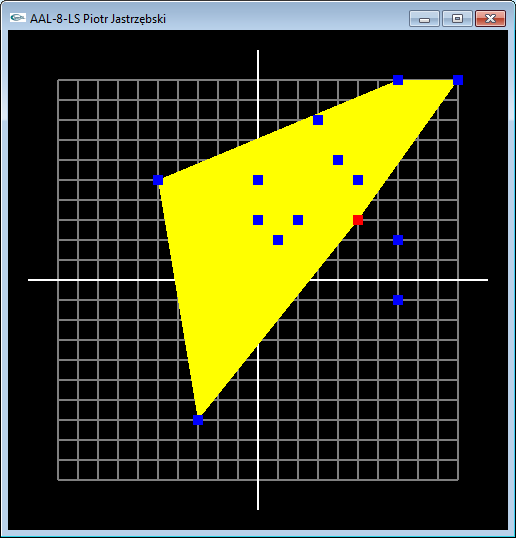
\includegraphics[width=\textwidth]{ss.png}
\caption{Zrzut ekranu. Wielokąt wypukły pokrywający największą liczbę punktów.}
\label{img_ss} 
\end{figure}

\section{Struktury danych}
Ze względu na klasę problemu, przechowywane dane ograniczają się do relacji dwu klas: klasy zbiorczej - Vertices oraz elementów tej klasy - punktów przechowywanych w klasie MyPoint.
\subsection{Klasa MyPoint}
Informacje oraz metody dotyczące pojedynczego punktu w układzie $XY$ (współrzędna $X$, współrzędna $Y$, fakt bycia punktem zaznaczonym) przechowywane są w klasie MyPoint. Jeśli punkt jest punktem wyróżnionym, isMarked przyjmuje wartość $true$.
\begin{verbatim}
class MyPoint{
private:
   double x;
   double y;
   bool isMarked;
public:
   MyPoint();
   MyPoint(double, double, bool);
   double getX();
   double getY();
   bool getIsMarked();
};
\end{verbatim}

\subsection{Klasa Vertices}
Informacje oraz metody zbioru punktów (np. zbiór wejściowy, wygenerowana otoczka wypukła, zbiór punktów do kreślenia wielokąta) przechowywane są w klasie Vertices.
\begin{verbatim}
class Vertices{
private:
   std::vector<class MyPoint> myVector;
public:
   void push(MyPoint);
   bool loadFromFile(std::string);
   std::vector<MyPoint> getMyVector();
   MyPoint getMyMarkedPoint();
   void setMyVector(std::vector<MyPoint>);
   void dumpContent(std::string name);
   bool isPointMarked(MyPoint);
   void clearVector();
   void generateRandom(int);
};
\end{verbatim}

\section{Algorytmy pomocnicze}
Jedynym pomocniczym algorytmem użytym w projekcie jest algorytm Jarvisa pozwalający na wyznaczanie otoczki wypukłej zbioru punktów na płaszczyźnie. Algorytm został podzielony na 2 części, co zostało przedstawione kolorami na rysunku \ref{img_jarvis}. Podążając dwoma drogami, od punktu o najmniejszych współrzędnych $(x,y)$ w górę oraz od punktu o największych współrzędnych $(x,y)$ w dół wyznaczane są dwa zbiory punktów. Konkatenacja tych zbiorów w rezultacie daje otoczkę wypukłą tworzącą wielokąt wypukły pokrywający największą liczbę punktów.

\begin{figure}
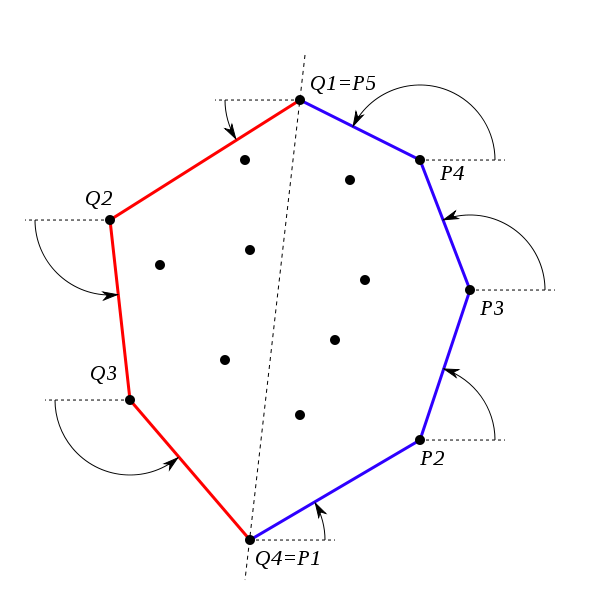
\includegraphics[width=\textwidth]{jarvis.png}
\caption{Schemat działania algorytmu Jarvisa.}
\label{img_jarvis}
\end{figure}

\section{Przewidywana złożoność}
\subsection{Maksymalna liczba wierzchołków wielokąta wypukłego}
Dla rozwiązania heurystycznego ze względu na możliwość niedeterministycznego zachowania złożoność może bardzo się zmieniać. Jednakowoż można przyjąć, że $O(T(n))=n^2$. Przy takim założeniu wyniki dla 30 instancji różnych zbiorów przedstawiono na rysunku \ref{img_3}.

Dla porównania, złożonością rozwiązania naiwnego można rozważyć jako liczbę wywołań kalkulacji otoczki wypukłej dla podzbioru. Tym samym dla zbioru $n$ elementowego należy rozważyć usuwanie od $0$ do $n-3$ (aby pozostały chociaż 3 punkty wymagane do stworzenia wielokąta) punktów spośród podzbioru $n-1$ ostatnich punktów (pierwszy jest nie usuwany, gdyż jest wyróżniony).
Z charakteru algorytmu wynika, że tworzy on wariacje bez powtórzeń z podzbioru, tym samym liczba obliczonych otoczek wyrażałaby się wzorem:
$\sum_{k=0}^{n-3} \frac{(n-1)!}{((n-1)-k)!}$, gdzie dominującym czynnikiem zapewne jest $(n-1)!$. Często podawanym przybliżeniem dla $n!$ jest, że dla każdego $n$ zachodzi nierówność: $(n/3)^n < n!$, a dla $n>6$: $(n/2)^n > n!$. Tym samym dla: $O(T(n))=((n-1)/3)^{n-1}$ otrzymuje się wyniki jak na rysunku \ref{img_1} (maksymalnie 8 wierzchołków). Za końcową złożoność dla dużych $n$ można przyjąć: $O(T(n))=n^n$.
\subsection{Maksymalna liczba punktów przykryta wielokątem wypukłym}
W związku z pętlą zagnieżdżoną w innej pętli, gdzie zbiór po którym odbywa się iteracja w obydwu przypadkach wynosi $n$, prognozuję złożoność obliczeniową jako $O(T(n))=n^2$. Wyniki otrzymane z testów, mimo obecności w pętlach różnie działających rezultatów spełnienia warunków logicznych potwierdzają złożoność. Przedstawiono je na rysunku \ref{img_2} dla maksymalnej liczby 100 wierzchołków.
\begin{figure}
\includegraphics[width=\textwidth]{3.png}
\caption{Wyniki dla wyszukiwania maksymalnej liczby wierzchołków. (heurystyczne)}
\label{img_3}
\end{figure}
\begin{figure}
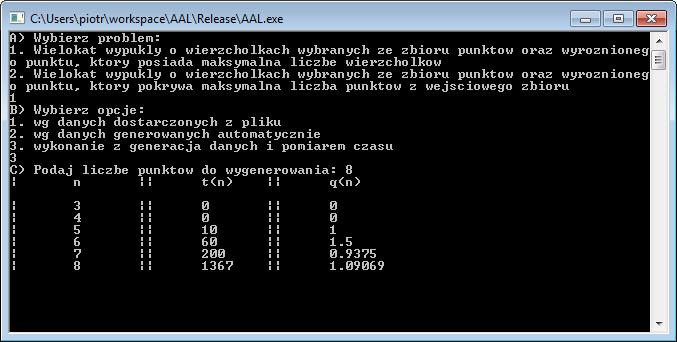
\includegraphics[width=\textwidth]{1.png}
\caption{Wyniki dla wyszukiwania maksymalnej liczby wierzchołków. (naiwne)}
\label{img_1}
\end{figure}
\begin{figure}
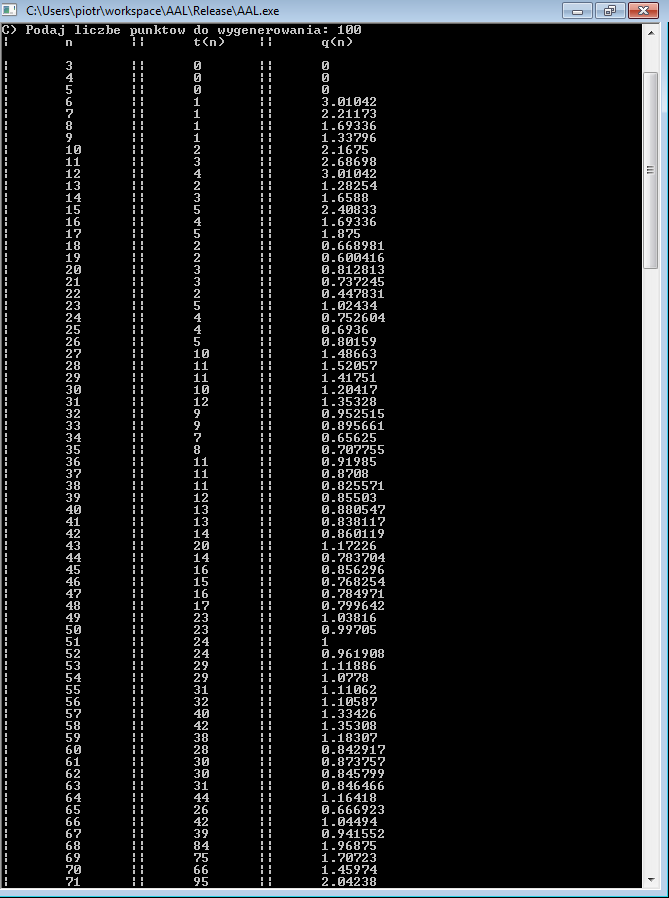
\includegraphics[width=\textwidth]{2.png}
\caption{Wyniki dla wyszukiwania największej liczby przykrytych punktów.}
\label{img_2}
\end{figure}

\end{document}